% \documentclass[letterpaper,12pt]{article}
\documentclass[a4paper,10pt]{article}
\usepackage[total={18cm,20cm}, top=1.5cm, left=1.5cm]{geometry}
\usepackage[spanish]{babel}
\renewcommand\spanishtablename{Tabla}
\usepackage[utf8]{inputenc}
%\usepackage[latin1]{inputenc}
\usepackage[T1]{fontenc}
\usepackage{caption}
\usepackage{graphicx}
\usepackage{subfigure}
\usepackage{fancyhdr}
\usepackage{setspace}
\usepackage{hyperref}
\usepackage{multirow}
\usepackage{float}

\renewcommand{\baselinestretch}{1.5}
\pagestyle{fancy}
\rhead{
\includegraphics[width = .055\textwidth]{imagenes/LogoBase.png}}
\lhead{\textit{Social Data Mining \& statistics}}

% \fancyfoot[R]{\includegraphics[width=5mm]{./imagenes/logo.png}}

\title{Comparando tiempos de publicación de redes sociales de automotrices. 
¿Cuáles son los mejores días y horas para publicar?}

\author{Social Data Mining \& Statistics \\
        Base10\\
        \scriptsize Dorantes Nieto Fernando ferdorantes@base10.mx \\
        \scriptsize Morán Titla Christian Daniel christian@base10.mx}

% \subtitle{LatReach}
\date{}


\begin{document}

\maketitle

%\begin{abstract}
%\end{abstract}

\section{Introducción}
De los cerca de 7,600 millones de personas que  actualmente viven en la Tierra, cerca
de la mitad (49.3\% ó 3,731,973,423 de personas) usan Internet como medio de comunicación (Internet World Stats, 2017),
el uso de internet incrementa con el paso de los años y de los muchos sitios web existentes
hay algunos cuya popularidad también va en aumento, tal es el caso de las redes sociales,
las cuales son  medios de comunicación que permiten la interacción 
de muchos individuos mediante el uso de la web.\\

Facebook es una de las redes sociales más populares (Smarthinsights, 2016) con cerca de
1,230 millones de usuarios activos diarios (Facebook statistics, 2017).
El propósito de Facebook es el de comunicar  a las personas, sin embargo
su uso va más allá y puede utilizarse con fines académicos o inclusive para el mercadeo (``Marketing'' en inglés) (Wilson et al, 2012).
En el caso concreto del mercadeo, el hecho de que las personas inviertan una buena cantidad de su tiempo en Facebook, 
permite que esta herramienta sea utilizada como un canal de anuncios para diversas marcas (Roshnee y Fowdar, 2013).
La gran cantidad de usuarios con ideas y costumbres diferentes permite a las empresas
realizar diversas estrategias específicas de mercadeo para sus potenciales clientes 
(Casteleyn et al, 2009).\\

El tiempo promedio que una persona pasa en Facebook es de 50 minutos al día (Stewart, 2016),
sin embargo las horas y días en las que una persona pasa en esta red social es diferente
con respecto a la zona geográfica y la ocupación de las personas, por lo que crear estrategias 
para postear (crear contenido en Facebook) también dependerá de estas variables.



Para el caso concreto de las redes sociales de SEAT y Volkswagen Financial Services
los ``Community managers'' de estas cuentas se esfuerzan en crear estrategias para postear y dar seguimiento a sus clientes,
es por ello que se requiere saber cuales son los mejores días y horas para postear, esta información ayudará a generar mejores estrategias
de mercadeo para sus clientes y fans.\\


Es por ello que el área de ciencia de datos en Base10 propone un experimento
para determinar la mejor hora y el mejor día para realizar posteos y de esta manera
tener una mejor interacción en Facebook con los clientes y fans de SEAT y Volkswagen Financial Services.


\section{Objetivo general}
Determinar la mejor hora y día para postear en Facebook.

\section{Objetivos particulares}
  \begin{itemize}
   \item[$*$] Conocer cual es la  mejor hora para postear en Facebook.
   \item[$*$] Conocer cual es el mejor día para postear en Facebook.
   \item[$*$] Comparar el tipo de contenido (imágenes o videos) que genera mejor interacción en Facebook.
   \item[$*$] Comparar las horas y días de las publicaciones para saber cuál de estas genera una  mayor interacción.
  \end{itemize}


\section{Materiales y métodos}
\subsection{Experimento}
El experimento consistió en obtener el número de posteos diarios de 12 perfiles
públicos de automotrices de Facebook (Tabla 1), dichos perfiles deberán ser solo de México, 
la temporalidad de los datos será de  2 años y 4 meses (2015-Abril de 2017).
Para cada perfil, se tomó en cuenta el tipo de posteo, la hora, el día, el mes y año de 
las publicaciones como variables independientes.\\
Las variables de respuesta son el número de comentarios,
el número de veces compartido y el número de reacciones de cada posteo (Figura 1),
para el caso del porcentaje de enganche de los posteos, se tomó en cuenta
la cuenta de Volkswagen Financial Services (https://www.facebook.com/vwfsmx/)
y la cuenta de SEAT, puesto que son las cuentas administradas por Base10 .


\begin{center}
\captionof{table} {Cuentas analizadas con el link adjunto. } \\[0.3cm] 
{\footnotesize
   \begin{tabular} {l|l|l} 
    \hline
    & Nombre Cuenta & Link \\ 
    \hline
    1 & Audi México & https://facebook.com/110458898990956 \\
    2 & BMW México & https://facebook.com/91610842685 \\
    3 & Chevrolet & https://facebook.com/198139706022 \\
    4 & Dodge México & https://facebook.com/358548171022 \\
    5 & Honda México & https://facebook.com/142339495886070 \\
    6 & Hyundai México & https://facebook.com/1452189031676518  \\
    7 & Kia Motors México & https://facebook.com/1499069493698389 \\
    8 & Mazda México &  https://facebook.com/694361250580489 \\
    9 & Nissan &  https://facebook.com/193593684019610 \\
    10 & SEAT México & https://facebook.com/113144262054871 \\
    11 & Toyota México & https://facebook.com/430457856994464 \\
    12 & Volkswagen & https://facebook.com/119666104757849 \\
    \hline
    \end{tabular}
}
\end{center}





\begin{figure}[H]
  \begin{center}
   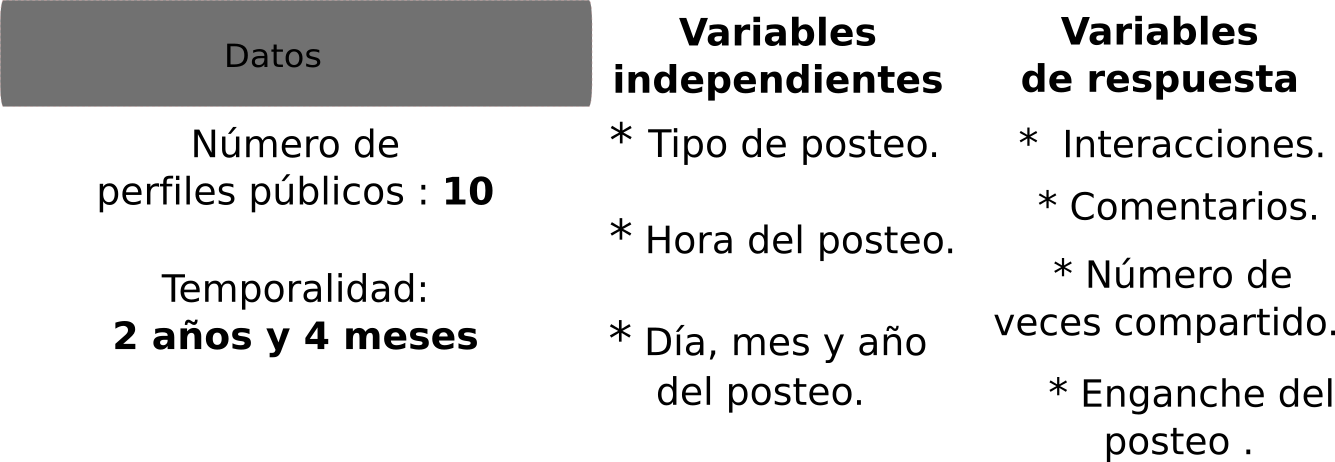
\includegraphics[width=.75\textwidth]{imagenes/figura1.png}
   \caption{Diseño experimental}
  \end{center} 
\end{figure}

\subsection{Colecta de datos}
Los datos de los perfiles de redes sociales se tomarán diréctamente de la API Graph de Facebook 
versión 2.9 (Facebook for developers, 2017), las llamadas a la API se realizaron con el lenguaje de programación Python
versión 2.7, y el paquete Rfacebook (Barbera et al, 2017) del lenguaje de programación R (R Core Team, 2017).

\subsection{Análisis estadísticos}
Las diferencias del número de reacciones, comentarios y veces compartido ``shares'' 
con respecto al tipo de publicación, hora y día del posteo sumando el efecto de
la fuente de los datos (cuenta de Facebook) fue analizado con un modelo mixto 
con distribución tipo ``poisson''.\\
Por otro lado para el caso del enganche y las impresiones, fueron 
analizadas separando por cuenta (SEAT y VWFS) tomando como variables
explicativas el número de posteos, el tipo de publicación, el día y hora de 
la publicación. Para hacer esta comparación, se realizaron modelos lineales generalizados (GLM)
con distribución quasibinomial con liga ``logit'', esto debido a que los residuales 
presentaron sobredispersión.
Cabe señalar que para  estos análisis no se tomaron en cuenta
los diferentes husos horarios presentes en México,
por lo que la hora estándar utilizada como hora de interacción 
fue la de la zona del centro de México (CENAM, 2017).
Todos los análisis estadísticos se realizaron con el lenguaje de programación
R (R Core Team 2017) en conjunto con los paquetes ``lme4'' (Bates et al 2015), 
ggplot2 (Wickham 2009), ``data.table'' (Dowle y Srinivasan 2017) y 
``dplyr'' (Wickham y Francois 2016). 



\section{Resultados}
\subsection{Resultados generales}
La cuenta con el mayor número de posteos fue SEAT con 3542 y la menor Nissan con 798 (Tabla 2).\\
El mayor número de interacciones fue de la cuenta Volkswagen con 19,298,782 y la 
menor Hyundai con  1,189,251 (Tabla 3).


\subsection{Días y horas}
El día con el mayor número de reacciones totales (suma de ``Me gusta'', 
``Me encanta'', ``Me entristece'', ``Me divierte'', ``Me enoja'', ``Me asombra'')
para todas las cuentas y en el mayor periodo de tiempo fue el día Martes ,
para el caso de los comentarios fue el Lunes y para el caso
de Número de veces compartido fue el Viernes, todos a las 20 horas (Figuras 2, 3 y 4).

De manera general el rango de horas de mayor actividad para todos los días
de la semana fue de 19 a 21 horas (Figuras 5 a 8), seguido del rango de 9 
a 12 horas. Tomando como los días de mayor actividad Miércoles a Viernes, 
con una baja actividad los fines de semana (Sábado y Domingo). 

Con respecto al  enganche para las cuentas SEAT y VWFS, el
mayor enganche lo presentaron el día Jueves a las 22 y 17 horas
respectivamente (Figuras 9 a 12).

El modelo mixto indica  que existe efecto del número
de posteos realizados, del tipo de posteo, de la hora y
del día del posteo (\textit{p}<0.05)  sobre el
total de reacciones, comentarios y número de veces compartido (Tablas 4 a 7).

El enganche de SEAT se ve afectado principalmente por
el número de posteos (71\% de la variación) seguido de 
la hora (6.1\%) (Tabla 8). Para el caso del enganche de VWFS el día de la
semana fue el que explica la mayor variación (25\%) seguido
de la hora (21\%) (Tabla 9).


\section{Discusión}
Puesto que facebook es una red social muy popular y su presencia es a nivel mundial, 
detectar una hora ideal para postear se ve sesgada a una región en particular, esto
debido a los diferentes husos horarios presentes en cada país.\\
Estos husos horarios pueden ser tomados en cuenta, como en el caso de Ellering (2016)
el cuál muestra un estudio donde se tomaron en cuenta los husos horarios
de Estados Unidos y para este país n concluye que el mejor horario para postear 
es de jueves a domingo si lo que  se desea es obtener un buen porcentaje de enganche, 
por otro lado si se desea obtener clicks, las 15 horas parecen ser la hora ideal.
Esto va de la mano con la cantidad de usuarios activos en la red social, 
que generalmente es de 12 a 22 horas. 
Fontein (2016) muestra que los mejores días para postear son los jueves y viernes
de 13 a 15 horas.\\
Estos resultados son parecidos a los nuestros para los fans de las cuentas
automotrices, puesto que se encontró que un buen horario para postear 
es en el intervalo de las 19 a 21 horas y de las 12 a las 15 horas. 
Los mejores días fueron los días lunes, martes, jueves y viernes,
esto para el caso de todas las automotrices. No obstante para realizar 
un mejor análisis sería conveniente tomar en cuenta el horario de actividad
de los fans de las cuentas, los husos horarios de los fans de las cuentas y
los sitios de origen de los fans, lo cual nos dará una mejor comprensión 
de la mejor opción de postear en Facebook.




\section{Conclusiones}
De manera general, las interacciones se ven afectadas por una gran 
cantidad de factores, tal es el caso de la hora y el día, 
las mayores interacciones se obtienen 
al postear entre las 18 a  21 horas y de las 12 a 15 horas, 
tomando en cuenta el posteo entre los días Lunes, Martes, Jueves y Viernes,
puesto que el fin de semana la interacción es mucho menor.\\
Para el caso del enganche, para VWFS la hora y el día
del posteo si tuvieron un efecto en el porcentaje de personas  enganchadas,
lo cual para el caso de SEAT cambia completamente
puesto que el número de posteos realizados por cada día
es mucho más influyente en el enganche.



\section{Anexos}
\subsection{Figuras}
\subsubsection{Figura 2}
\begin{figure}[H]
  \begin{center}
   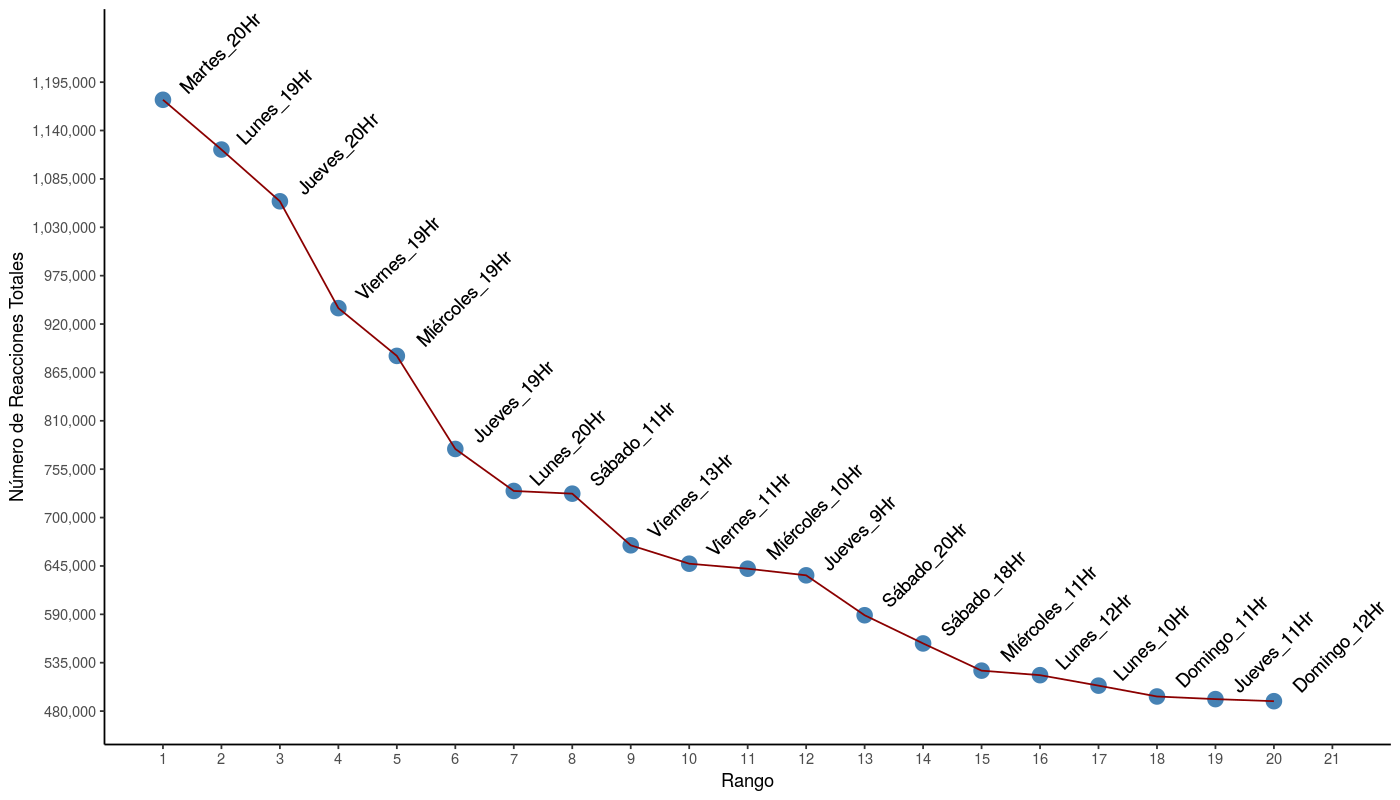
\includegraphics[width=.85\textwidth]{imagenes/figura2.png}
   \captionsetup{width=.80\textwidth}
   \caption{\centering Dias y horas con el mayor número de reacciones totales en el rango de tiempo
   comprendido del 1 de Enero de 2015 al 30 de Abril de 2016 (Se muestran los  20 más abundantes).}
  \end{center} 
\end{figure}

\subsubsection{Figura 3}
\begin{figure}[H]
  \begin{center}
   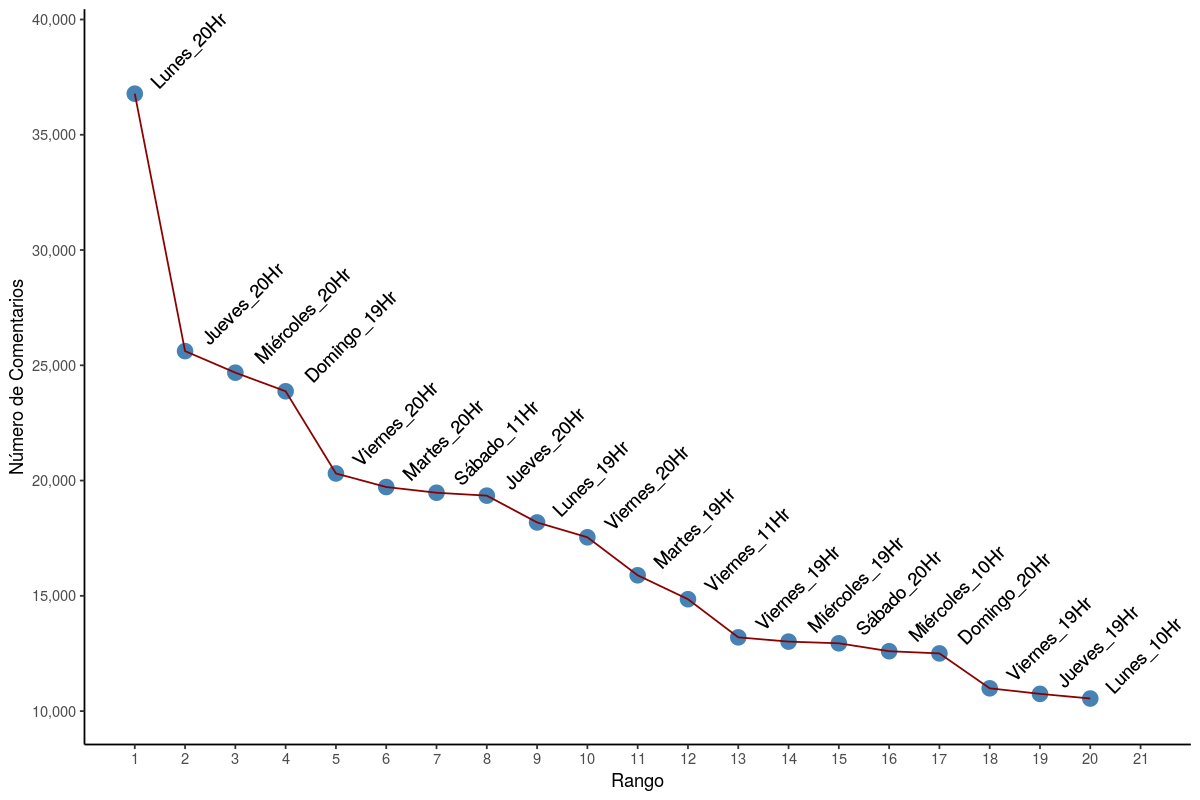
\includegraphics[width=.85\textwidth]{imagenes/figura3.png}
   \captionsetup{width=.80\textwidth}
   \caption{\centering Dias y horas con el mayor número de comentarios.} 
   \end{center} 
\end{figure}

\subsubsection{Figura 4}
\begin{figure}[H]
  \begin{center}
    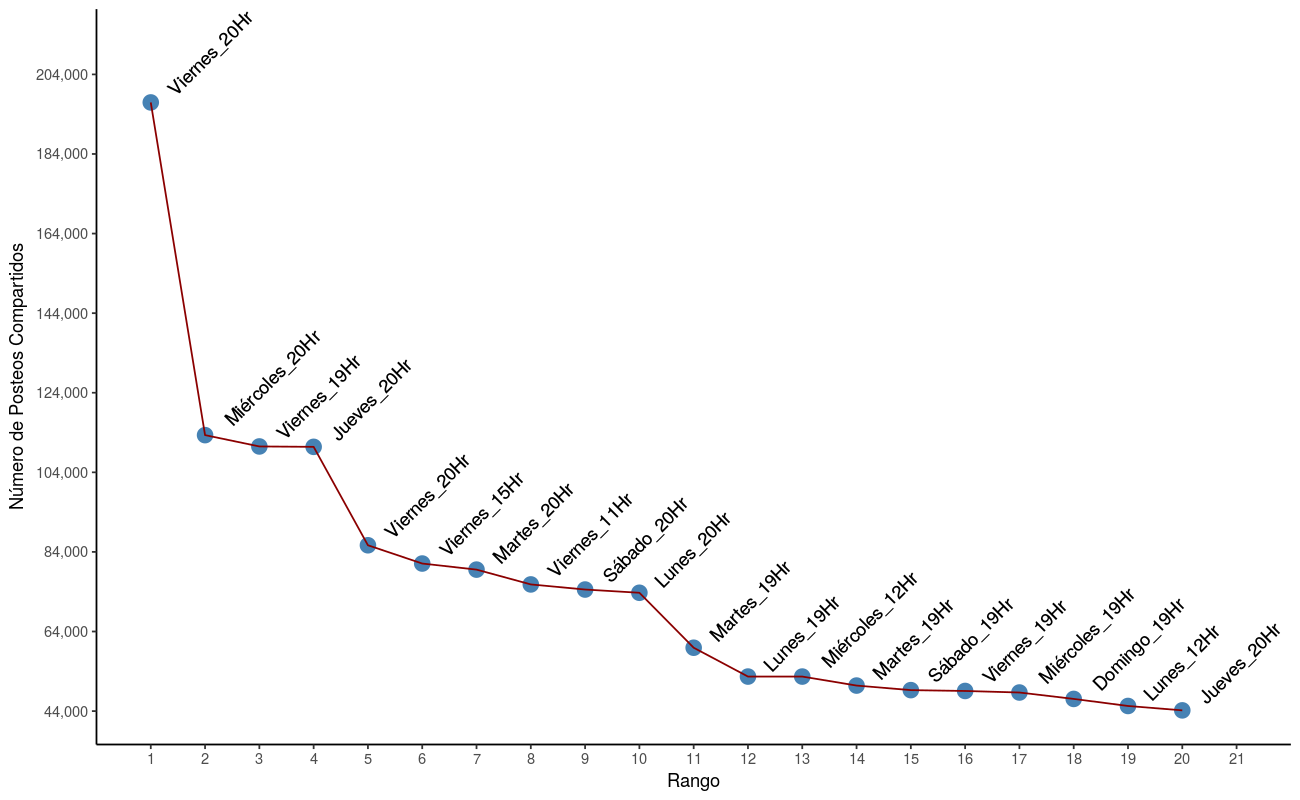
\includegraphics[width=.85\textwidth]{imagenes/figura4.png}
    \captionsetup{width=.80\textwidth}
    \caption{\centering Dias y horas con el mayor número de posteos compartidos.}   
   \end{center} 
\end{figure}

\subsubsection{Figura 5}
\begin{figure}[H]
  \begin{center}
   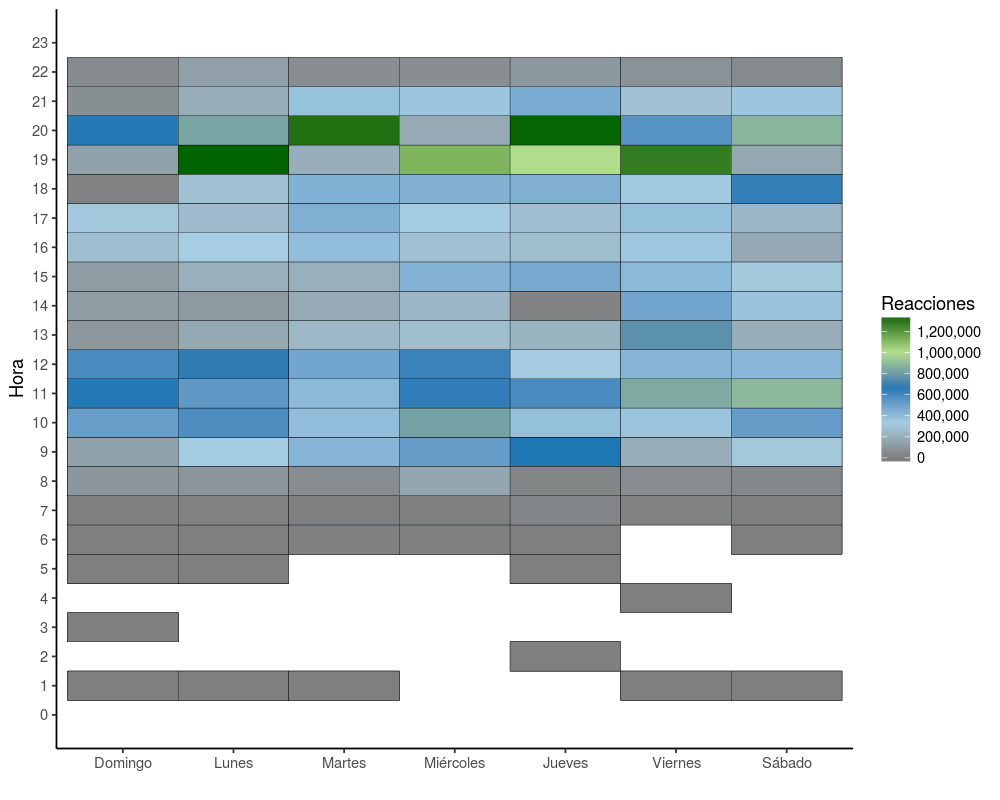
\includegraphics[width=.85\textwidth]{imagenes/figura5.png}
   \captionsetup{width=.80\textwidth}
   \caption{\centering Concentración de interacciones totales 
   (Suma de reacciones, comentarios y número de veces compartido) durante el día y a 
   lo largo de la semana.} 
  \end{center} 
\end{figure}


\subsubsection{Figura 6}
\begin{figure}[H]
  \begin{center}
   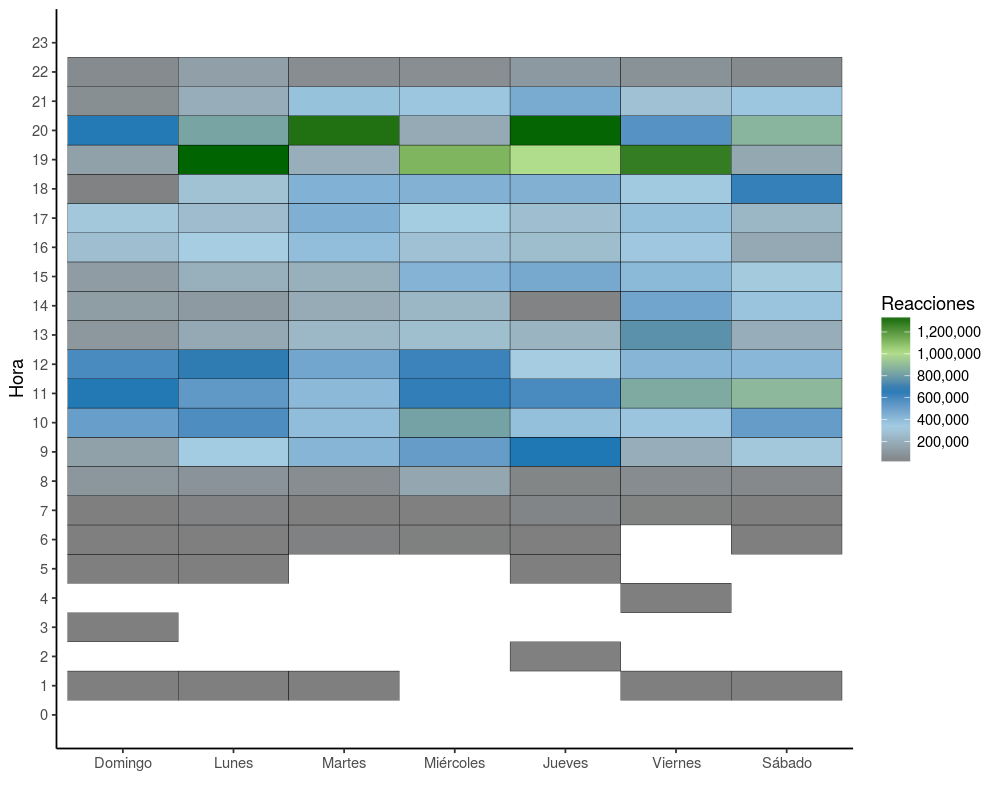
\includegraphics[width=.85\textwidth]{imagenes/figura6.png}
   \captionsetup{width=.80\textwidth}
   \caption{\centering Concentración de reacciones totales durante el día y a 
   lo largo de la semana.} 
  \end{center} 
\end{figure}

\subsubsection{Figura 7}
\begin{figure}[H]
  \begin{center}
   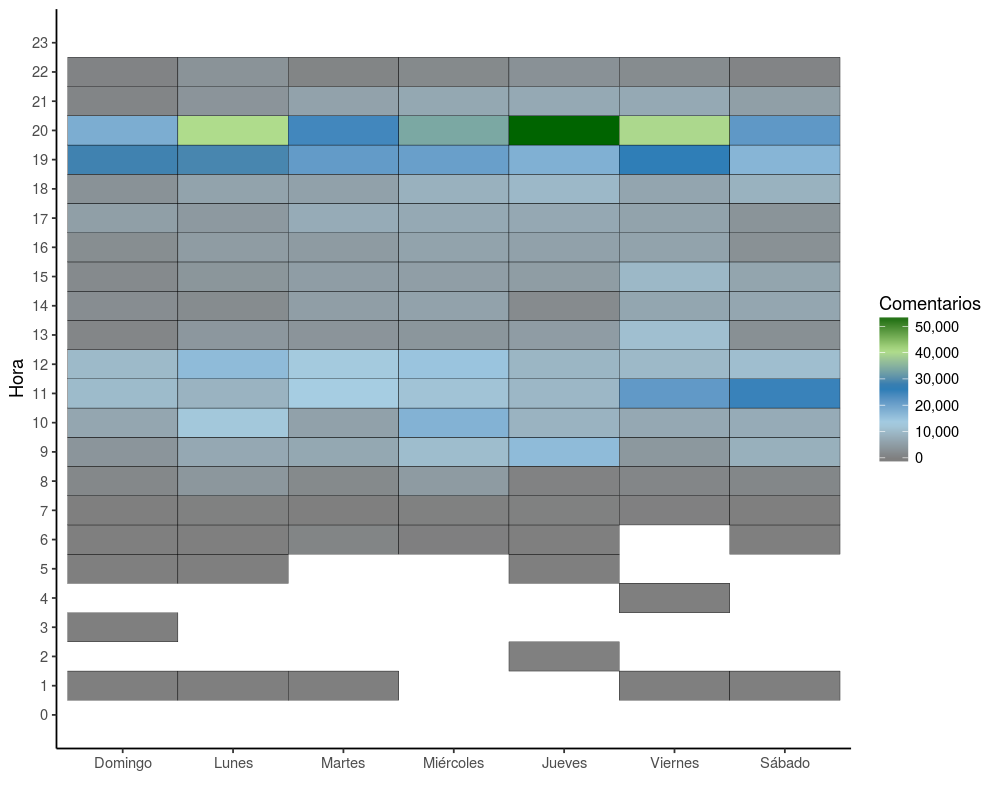
\includegraphics[width=.85\textwidth]{imagenes/figura7.png}
   \captionsetup{width=.80\textwidth}
   \caption{\centering Concentración de comentarios durante el día y a 
   lo largo de la semana.} 
  \end{center} 
\end{figure}

\subsubsection{Figura 8}
\begin{figure}[H]
  \begin{center}
   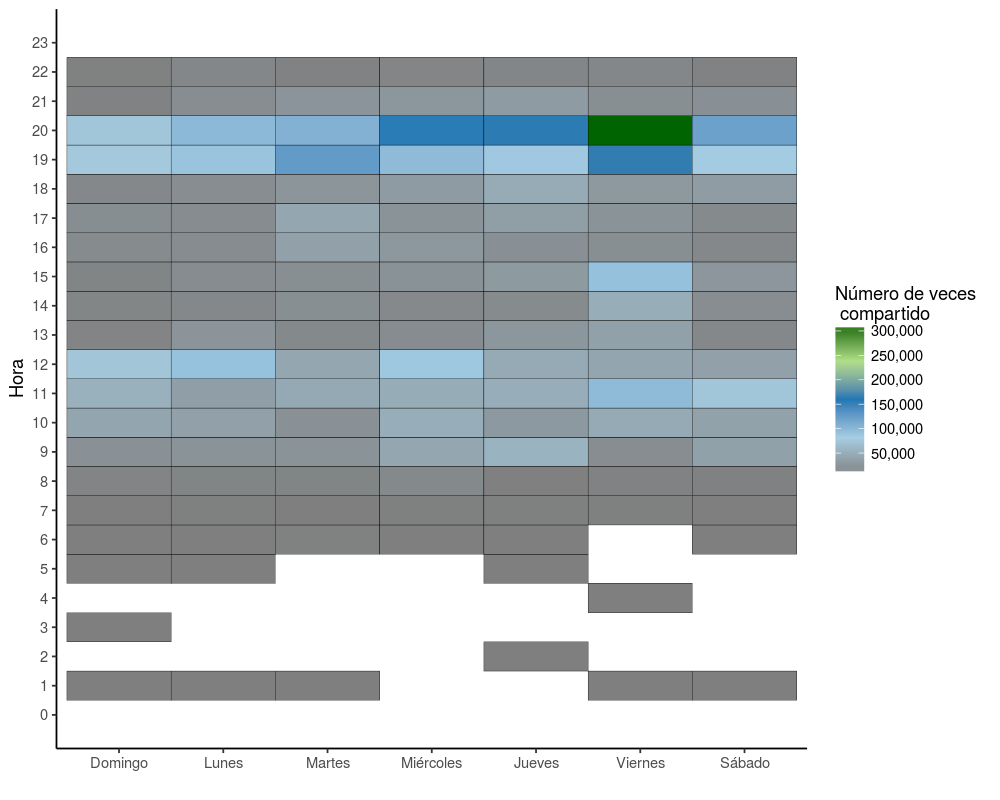
\includegraphics[width=.85\textwidth]{imagenes/figura8.png}
      \captionsetup{width=.80\textwidth}
   \caption{\centering Concentración de número de posteos compartidos totales durante el día y a 
   lo largo de la semana.} 
  \end{center} 
\end{figure}

\subsubsection{Figura 9}
\begin{figure}[H]
  \begin{center}
   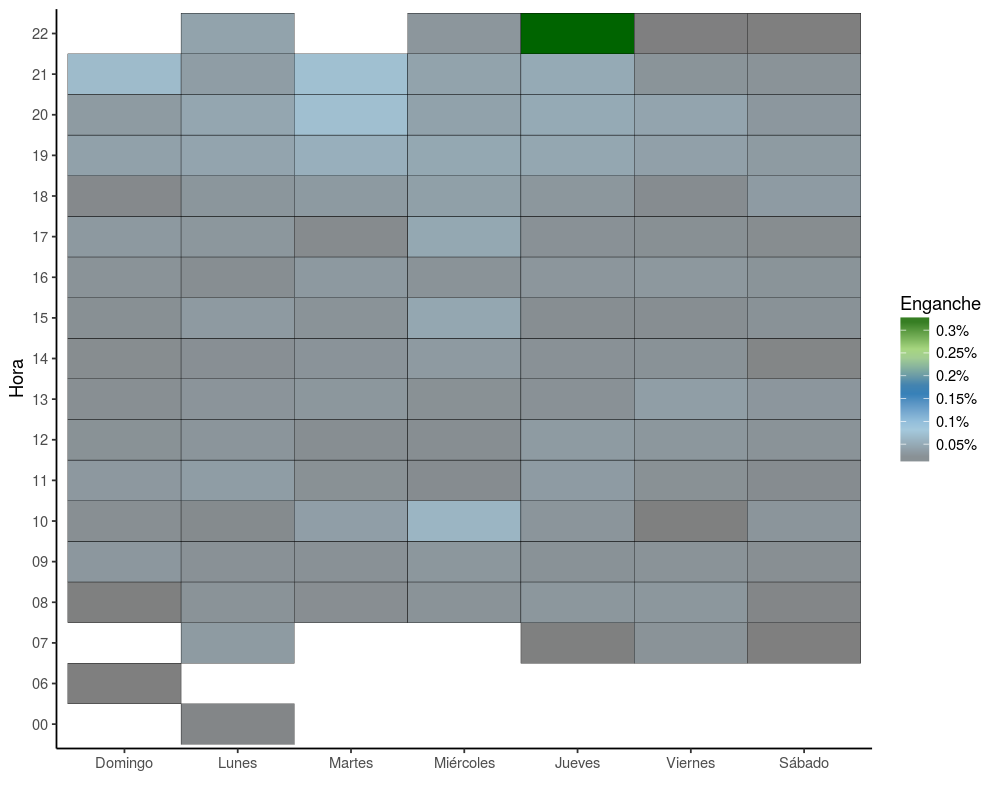
\includegraphics[width=.85\textwidth]{imagenes/figuraEnganche1.png}
      \captionsetup{width=.80\textwidth}
   \caption{\centering Promedio del porcentaje de enganche para la cuenta de SEAT.} 
  \end{center} 
\end{figure}

\subsubsection{Figura 10}
\begin{figure}[H]
  \begin{center}
   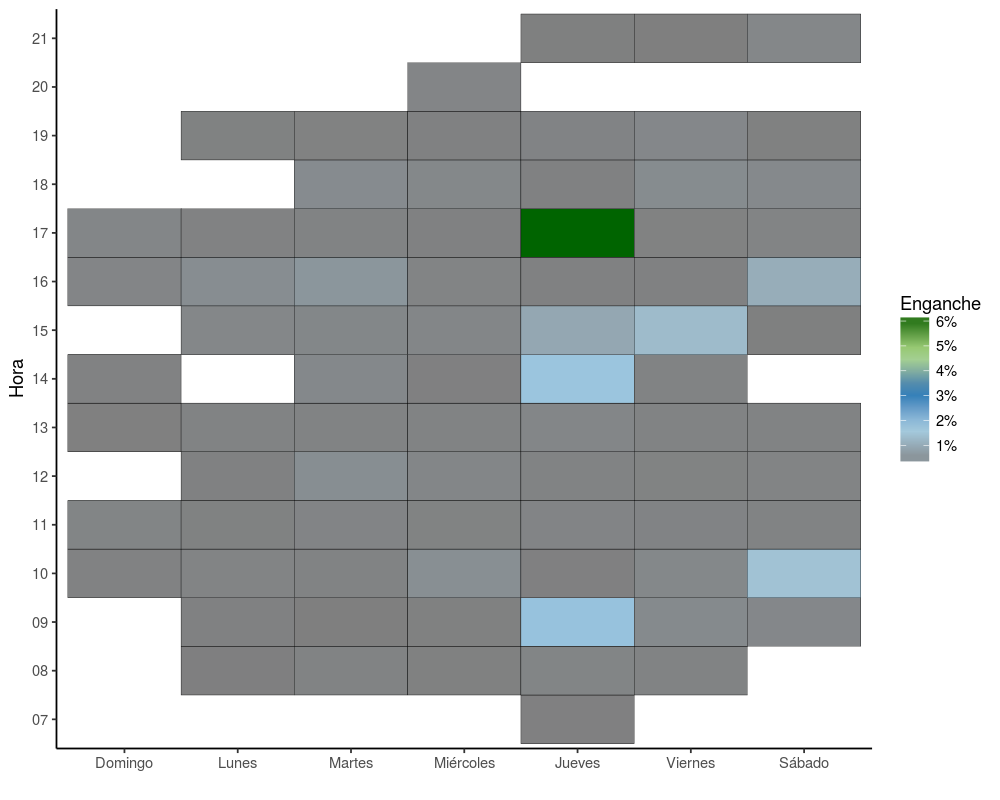
\includegraphics[width=.85\textwidth]{imagenes/figuraEnganche2.png}
      \captionsetup{width=.80\textwidth}
   \caption{\centering Promedio del porcentaje de enganche para la cuenta de VWFS.} 
  \end{center} 
\end{figure}

\subsubsection{Figura 11}
\begin{figure}[H]
  \begin{center}
   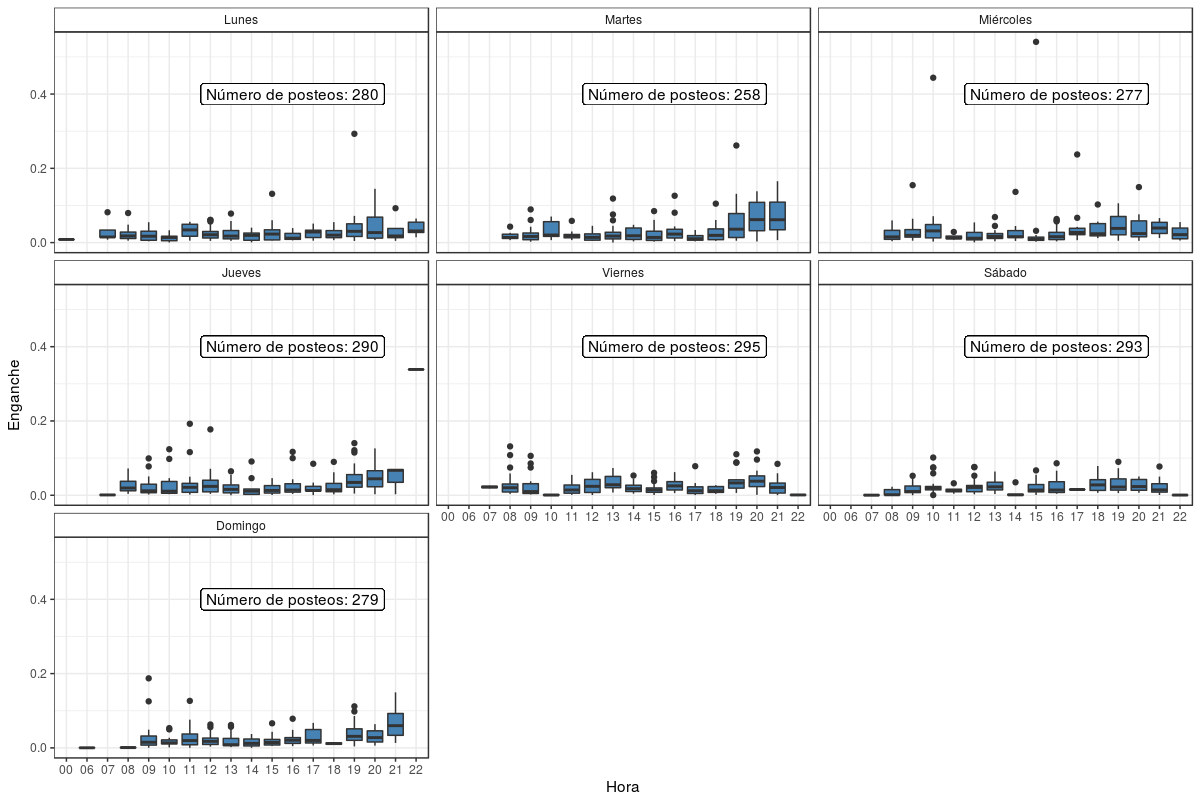
\includegraphics[width=.85\textwidth]{imagenes/engancheSeat}
      \captionsetup{width=.80\textwidth}
   \caption{\centering } 
  \end{center} 
\end{figure}


\subsubsection{Figura 12}
\begin{figure}[H]
  \begin{center}
   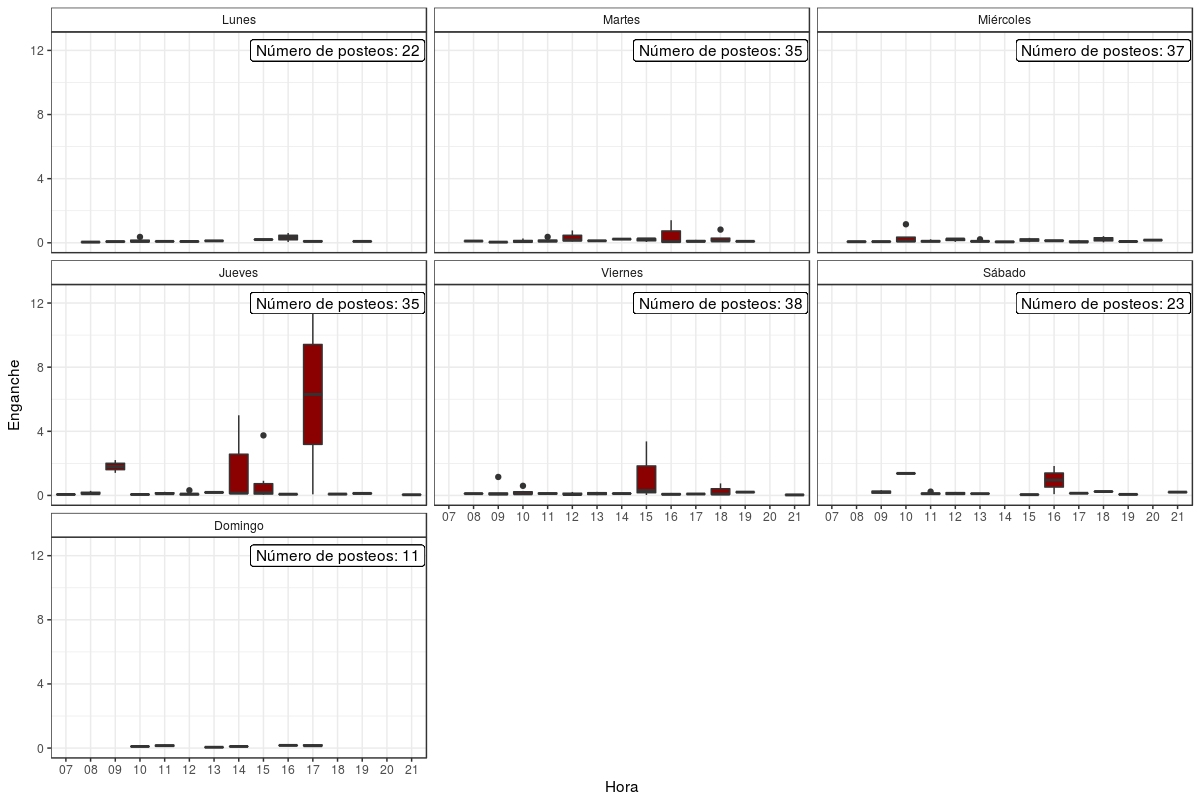
\includegraphics[width=.85\textwidth]{imagenes/engancheVwfs}
      \captionsetup{width=.80\textwidth}
   \caption{\centering } 
  \end{center} 
\end{figure}


\subsection{Tablas}

\subsubsection{Tabla 2}

\begin{center}
  \captionof{table}{Número de posteos por cuenta.}\\[0.3cm]
  \begin{tabular}{l|l|c}
    \hline 
    & Cuenta & Número de posteos \\
    \hline
    1 & Audi de México & 1794 \\
    2 & BMW Mexico & 993 \\
    3 & Chevrolet & 930 \\
    4 & Dodge México & 854 \\
    5 & Honda México & 1344 \\
    6 & Hyundai México & 1101 \\
    7 & Kia Motors México & 1715 \\
    8 & Mazda México & 1505 \\
    9 & Nissan & 798 \\
    10 & SEAT México & 3542 \\
    11 & Toyota México & 1032 \\
    12 & Volkswagen & 1421 \\
    \hline
  \end{tabular}
\end{center}

\subsubsection{Tabla 3}

\begin{center}
  \captionof{table}{Número de interacciones por cuenta.}\\[0.3cm]
  \begin{tabular}{l|l|c}
    \hline
    & Cuenta & Número de interacciones \\
    \hline
    1 & Audi de México & 3,842,344 \\
    2 & BMW Mexico & 2,103,275 \\
    3 & Chevrolet & 4,258,177 \\
    4 & Dodge México & 1,735,909 \\
    5 & Honda México & 1,978,830 \\
    6 & Hyundai México & 1,189,251 \\
    7 & Kia Motors México & 5,380,232 \\
    8 & Mazda México & 4,164,856 \\
    9 & Nissan & 2,438,827 \\
    10 & SEAT México & 1,874,289 \\
    11 & Toyota México & 4,272,703 \\
    12 & Volkswagen & 19,298,782 \\
    \hline
  \end{tabular}
\end{center}



\subsubsection{Tabla 4}
\begin{center}
  \captionof{table}{Resumen del modelo mixto generalizado de las interacciones totales. }\\[0.3cm]
  \begin{tabular}{l|l|c|c|c|c}
    \hline
    & Factor & Estimado & Error estándar & Valor de \textit{P} & Tipo de factor\\
    \hline
    1 & Ordenada & 4.4697093 & 0.0978632 & < 0.001 & Fijo \\
    2 & Tipo Gif/Link & 2.9667910 & 0.0321940 & < 0.001 & Fijo \\
    3 & Tipo Foto & 3.1447253 & 0.0321907 & < 0.001 & Fijo \\
    4 & Tipo Estatus & 0.9909772 & 0.0324501 & < 0.001 & Fijo \\
    5 & Tipo Video & 2.9509620 & 0.0321921 & < 0.001 & Fijo \\
    6 & Día Jueves & -0.0268273 & 0.0022629 & < 0.001 & Fijo \\
    7 & Día Lunes & -0.1857828 & 0.0022620 & < 0.001 & Fijo \\
    8 & Día Martes & -0.3055006 & 0.0023193 & < 0.001 & Fijo \\
    9 & Día Miércoles & 0.5501174 & 0.0021720 & < 0.001 & Fijo \\
    10 & Día Sábado & -0.3345351 & 0.0022872 & < 0.001 & Fijo \\
    11 & Día Viernes & -0.4200540 & 0.0022094 & < 0.001 & Fijo \\
    12 & Hora & 0.0120595 & 0.0001092 & < 0.001 & Fijo \\
    13 & Día Jueves:Hora & 0.0034219 & 0.0001418 & < 0.001 & Fijo \\
    14 & Día Lunes:Hora & 0.0143518 & 0.0001430 & < 0.001 & Fijo \\
    15 & Día Martes:Hora & 0.0261333 & 0.0001442 & < 0.001 & Fijo \\
    16 & Día Miércoles:Hora & -0.0238167 & 0.0001379 & < 0.001 & Fijo \\
    17 & Día Sábado:Hora & 0.0188871 & 0.0001447 & < 0.001 & Fijo \\
    18 & Día Viernes:Hora & 0.0363681 & 0.0001382 & < 0.001 & Fijo \\
    19 & Cuenta & 0.7597790 &  &  & Aleatorio \\
    \hline
  \end{tabular}
\end{center}

\subsubsection{Tabla 5}
\begin{center}
 \captionof{table}{Resumen del modelo mixto generalizado de las reacciones totales. }\\[0.3cm]
  \begin{tabular}{l|l|c|c|c|c}
     \hline
    & Factor & Estimado & Error estándar & Valor de \textit{P} & Tipo de factor\\
    \hline
    1 & Ordenada & 4.4013972 & 0.0892075 & < 0.001 & Fijo \\
    2 & typelink & 2.9097964 & 0.0346406 & < 0.001 & Fijo \\
    3 & typephoto & 3.1484458 & 0.0346363 & < 0.001 & Fijo \\
    4 & typestatus & 0.9563817 & 0.0348913 & < 0.001 & Fijo \\
    5 & typevideo & 2.7670169 & 0.0346380 & < 0.001 & Fijo \\
    6 & Día Jueves & 0.0051029 & 0.0023769 & 0.0318 & Fijo \\
    7 & Día Lunes & -0.1592056 & 0.0023730 & < 0.001 & Fijo \\
    8 & Día Martes & -0.2847935 & 0.0024310 & < 0.001 & Fijo \\
    9 & Día Miércoles & 0.5630974 & 0.0022792 & < 0.001 & Fijo \\
    10 & Día Sábado & -0.3124751 & 0.0024013 & < 0.001 & Fijo \\
    11 & Día Viernes & -0.3722196 & 0.0023278 & < 0.001 & Fijo \\
    12 & Hora & 0.0134707 & 0.0001147 & < 0.001 & Fijo \\
    13 & Día Jueves:Hora & 0.0005212 & 0.0001491 & < 0.001 & Fijo \\
    14 & Día Lunes:Hora & 0.0121838 & 0.0001501 & < 0.001 & Fijo \\
    15 & Día Martes:Hora & 0.0248435 & 0.0001512 & < 0.001 & Fijo \\
    16 & Día Miércoles:Hora & -0.0248731 & 0.0001447 & < 0.001 & Fijo \\
    17 & Día Sábado:Hora & 0.0176629 & 0.0001520 & < 0.001 & Fijo \\
    18 & Día Viernes:Hora & 0.0313026 & 0.0001458 & < 0.001 & Fijo \\
    19 & Cuenta & 0.7461024 &  &  & Aleatorio \\
    \hline
  \end{tabular}
\end{center}

\subsubsection{Tabla 6}
\begin{center}
  \captionof{table}{Resumen del modelo mixto generalizado del número de comentarios totales. }\\[0.3cm]
  \begin{tabular}{l|l|c|c|c|c}
     \hline	
    & Factor & Estimado & Error estándar & Valor de \textit{P} & Tipo de factor\\
    \hline
    1 & Ordenada & 0.4235452 & 0.2594847 & 0.102 & Fijo \\
    2 & typelink & 2.3448420 & 0.1452266 & < 0.001 & Fijo \\
    3 & typephoto & 2.0705932 & 0.1451995 & < 0.001 & Fijo \\
    4 & typestatus & 1.2516872 & 0.1462334 & < 0.001 & Fijo \\
    5 & typevideo & 2.4870335 & 0.1452078 & < 0.001 & Fijo \\
    6 & Día Jueves & 0.3690978 & 0.0171882 & < 0.001 & Fijo \\
    7 & Día Lunes & 0.2292758 & 0.0170176 & < 0.001 & Fijo \\
    8 & Día Martes & 0.8856001 & 0.0175766 & < 0.001 & Fijo \\
    9 & Día Miércoles & 1.6931788 & 0.0164331 & < 0.001 & Fijo \\
    10 & Día Sábado & 0.8840528 & 0.0171651 & < 0.001 & Fijo \\
    11 & Día Viernes & 0.3630633 & 0.0169744 & < 0.001 & Fijo \\
    12 & Hora & 0.0630851 & 0.0008208 & < 0.001 & Fijo \\
    13 & Día Jueves:Hora & -0.0132651 & 0.0010349 & < 0.001 & Fijo \\
    14 & Día Lunes:Hora & 0.0000359 & 0.0010310 & 0.9721 & Fijo \\
    15 & Día Martes:Hora & -0.0538450 & 0.0010744 & < 0.001 & Fijo \\
    16 & Día Miércoles:Hora & -0.0959447 & 0.0010173 & < 0.001 & Fijo \\
    17 & Día Sábado:Hora & -0.0602103 & 0.0010653 & < 0.001 & Fijo \\
    18 & Día Viernes:Hora & -0.0147150 & 0.0010285 & < 0.001 & Fijo \\
    19 & Cuenta & 0.8725728 &  &  & Aleatorio \\
    \hline
  \end{tabular}
\end{center}


\subsubsection{Tabla 7}
\begin{center}
  \captionof{table}{Resumen del modelo mixto generalizado del número de ``Shares'' totales. }\\[0.3cm]
  \begin{tabular}{l|l|c|c|c|c}
    \hline
    & Factor & Estimado & Error estándar & Valor de \textit{P} & Tipo de factor\\
    \hline
    1 & Ordenada & -10.2355094 & 0.2094106 & < 0.001 & Fijo \\
    2 & typelink & 15.3472588 & 0.1418068 & < 0.001 & Fijo \\
    3 & typephoto & 14.9126134 & 0.1418025 & < 0.001 & Fijo \\
    4 & typestatus & 12.4376677 & 0.1430408 & < 0.001 & Fijo \\
    5 & typevideo & 15.9726640 & 0.1418029 & < 0.001 & Fijo \\
    6 & Día Jueves & -0.4456281 & 0.0081965 & < 0.001 & Fijo \\
    7 & Día Lunes & -0.4913703 & 0.0083773 & < 0.001 & Fijo \\
    8 & Día Martes & -0.8173742 & 0.0086477 & < 0.001 & Fijo \\
    9 & Día Miércoles & 0.1367379 & 0.0080057 & < 0.001 & Fijo \\
    10 & Día Sábado & -0.8598023 & 0.0084114 & < 0.001 & Fijo \\
    11 & Día Viernes & -0.9668135 & 0.0077747 & < 0.001 & Fijo \\
    12 & Hora & -0.0117634 & 0.0004007 & < 0.001 & Fijo \\
    13 & Día Jueves:Hora & 0.0382899 & 0.0005137 & < 0.001 & Fijo \\
    14 & Día Lunes:Hora & 0.0369934 & 0.0005316 & < 0.001 & Fijo \\
    15 & Día Martes:Hora & 0.0582518 & 0.0005361 & < 0.001 & Fijo \\
    16 & Día Miércoles:Hora & 0.0057486 & 0.0005086 & < 0.001 & Fijo \\
    17 & Día Sábado:Hora & 0.0503054 & 0.0005323 & < 0.001 & Fijo \\
    18 & Día Viernes:Hora & 0.0923213 & 0.0004851 & < 0.001 & Fijo \\
    19 & Cuenta & 0.9266213 &  &  & Aleatorio \\
    \hline
  \end{tabular}
\end{center}

\subsubsection{Tabla 8}

\begin{center}
  \captionof{table}{Tabla de devianza con los porcentajes de variación de los factores analizados para 
  el enganche de SEAT.}\\[0.3cm]
  \begin{tabular}{l|l|c|c|c}
    & Nombre & Devianza & Porcentaje de influencia & Gl \\
    \hline
    1 & Número Posteos & 0.645 & 71.501\% & 1 \\
    2 & Hora & 0.055 & 6.197\% & 17 \\
    3 & DiaSemana & 0.015 & 1.678\% & 6 \\
    4 & Error &  & 20.622\% &  \\
    \hline
  \end{tabular}
\end{center}

\subsubsection{Tabla 9}

\begin{center}
 \captionof{table}{Tabla de devianza con los porcentajes de variación de los factores analizados para 
  el enganche de VWFS.}\\[0.3cm]
  \begin{tabular}{l|l|c|c|c}
    & Nombre & Devianza & Porcentaje de influencia & Gl \\
    \hline
    2 & Número Posteos & 0.158 & 10.291\% & 1 \\
    3 & Hora & 0.324 & 21.006\% & 14 \\
    4 & DiaSemana & 0.385 & 24.997\% & 6 \\
    5 & Error &  & 43.704\% &  \\
    \hline
  \end{tabular} 
\end{center}

 
\\[2cm]

\begin{thebibliography}{20}
  \bibitem{1}  Bates D; Maechler M; Bolker B; Walker S. (2015). Fitting Linear Mixed-Effects Models Using lme4. Journal of Statistical Software,67(1), 1-48. doi:10.18637/jss.v067.i01.
  \bibitem{2} Casteleyn J; Mottart A; Rutten K. (2009). How to use Facebook in you market research. International Journal of Market Research. 51(4) 439-447.
  \bibitem{3} Centro Nacional de Metrología (CENAM) (2017). Tomado de: http://www.cenam.mx/
  \bibitem{4}  Dowle M; Srinivasan A. (2017). data.table: Extension of  data.frame. R package version 1.10.4. https://CRAN.R-project.org/package=data.table
  \bibitem{5}  Ellering N. (2016). What 16 Studies Say About The Best Times To Post On Social Media. Tomado de: https://coschedule.com/blog/best-times-to-post-on-social-media/.
  \bibitem{6} Facebook. (2017). \textit{ Statistics of  Facebook}, Palo  Alto,  CA:  Facebook. Tomado de: http://ltam.newsroom.fb.com/company-info/
  \bibitem{7} Facebook for developers (2017). Tomado de: https://developers.facebook.com/docs/graph-api
  \bibitem{8}  Fontein D (2016). El mejor momento para postear en redes sociales. Tomado de: https://blog.hootsuite.com/es/mejor-momento-publicar-redes-sociales/
  \bibitem{9}  Wickham H; Francois R. (2016). dplyr: A Grammar of Data Manipulation. R package version 0.5.0. https://CRAN.R-project.org/package=dplyr
  \bibitem{10}  Wickham H. (2009). ggplot2: Elegant Graphics for Data Analysis. Springer-Verlag Nueva York
  \bibitem{11} Internet World Stats. (2017). Tomado de: http://www.internetworldstats.com/stats.htm
  \bibitem{12} R Core Team (2017). R: A language and environment for statistical computing. R Foundation for Statistical Computing, Vienna, Austria. URL https://www.R-project.org/
  \bibitem{13} Roshnee R; Fowdar S. (2013). The implications of Facebook Marketing for Organizations. Contemporay Management Research. 9 (1) 73-84. doi:10.7903/cmr.9710 
  \bibitem{14} Smarth Insights. (2016). Global social media research summary 2016. Tomado de: http://www.smartinsights.com/social-media-marketing/social-media-strategy/new-global-social-media-research/
  \bibitem{15} Stewart J. (2017). Facebook Has 50 Minutes of Your Time Each Day. It Wants More. Tomado de : https://www.nytimes.com/2016/05/06/business/facebook-bends-the-rules-of-audience-engagement-to-its-advantage.html
  \bibitem{16}  Wilson R; Gosling S; Graham L. (2012). A review of Facebook research in the social sciences. Perspectives on Psychological Science 7 (3) 203-220
\end{thebibliography}


\end{document}
